\documentclass{article}

\usepackage{listings}
\usepackage{color}
\usepackage{fancyhdr}
\usepackage{graphicx}


\lstset{language=C,
  commentstyle=\color{red},
  keywordstyle=\color{blue}}

\begin{document}

\pagestyle{fancy}

\lfoot{\'Equipe 7381} 
\rfoot{Projet C - Semestre 5} 

\title{Rapport Projet C - Semestre 5}

\author{DUCOS Joris, DOULIERY Baudouin}
\date{}
\maketitle
\begin{center}
  \centering
  \huge
  \textbf{Atomic Teddy Investors} \\
  
\includegraphics[scale=1]{teddy.png}
  \end{center}
\begin{figure}[t]
  \centering
  
\includegraphics[scale=0.1]{Logo_INPB.png}
\end{figure}


\newpage
\newpage

\tableofcontents

\newpage


\section{Introduction}
\subsection{Contexte}
Ce rapport a pour objectif de pr\'esenter et d'expliquer le travail r\'ealis\'e sur le premier projet de programmation, en premi\'ere ann\'ee \`a l'ENSEIRB-MATMECA.
Le projet porte sur l'impl\'ementation d'un jeu, Atomic Teddy Investors, en langage C.On r\'ealise dans un premier temps une version de base, puis un ensemble d'achievement.

\subsection{Pr\'esentation du sujet}

Extrait de \textcolor{red}{\textit{Atomic Teddy Investors :}}\\ 

\textit{"La Sicile a \'et\'e finalement envahie, et les ours ont vaincu l'arm\'ee du Grand-Duc. Se m\^elant aux humains, ils se m\^elent aux divers aspects de la soci\'et\'e, 
reprenant \`a leur compte les divers m\'etiers propres \`a la race humaine. L'un des aspects qui les fascine est celui de l'\'economie de march\'e. Sur les places de 
march\'e de l'\^ile, ils se mettent \`a jouer les magnats, les barons, les grands seigneurs, afin d'arrondir leur p\'ecule personnel ventripotent. Dans leurs costumes 
impeccables, ils prospectent les villes \`a la recherche d'opportunit\'es d'achat et de revente, dans un but finalement assez simple : du miel, rien que du miel. 
Leur app\^at du gain est certainement plus gourmand que cupide, et on admettra que leur compr\'ehension de la m\'ecanique \'economique reste un peu hasardeuse, ce qui 
donne l'objet de ce sujet, qui d\'ecrit ces ensembles d'\'echanges \`a la mani\`ere d'un jeu."}


\subsection{Probl\'ematique}

Le but principal du projet est d'impl\'ementer le jeu, en langage C. Le probl\'eme principal du jeu est donc de g\'erer les choix des joueurs, pour qu'ils aient le plus de ressources. Donc on peut se demander comment les differents \'elements du jeu  vont \^etre mod\'elis\'es ?
Comment la boucle de jeu va fonctionner ? Comment les r\'egles du jeu vont \^etre respect\'ees ?
Tout ces probl\'emes vont \^etre divis \'es en sous-probl\'emes, afin de faciliter le travail. 

\section{M\'ethode}

\subsection{R\'epartition des t\^aches}
R\'epartion des t\^aches par sous-probl\'emes 
Chaque membre travail sur des sous-probl\'eme, afin d'avancer le plus vite possible.    

\subsection{Outils utilis\'es}

\subsubsection{D\'ep\^ot (forge)}

Le partage des fichiers c'est fait en utilisant le syt\`eme de d\^epot Thor, mis en place par nos professeurs encadrant. 
L'utilisation de git a permis d'envoyer les fichiers sur le d\^epot Thor, et ainsi d'\'echanger les informations entre co\`equipier.
Le d\^epot permet aussi de faire passer des test \`a nos fichiers, et ainsi de verifier que tout fonctionne correctement. 

\subsubsection{\'Editeur de codes}
L'int\'egralit\'e du projet est r\'ealis\'e en langage C.
Les logiciels comme Emacs, premettent d'\'editer les codes. 

\subsubsection{\LaTeX}

Ce rapport est r\'edig\'e en \LaTeX. Les fichiers relatifs \`a son \'ecriture sont pr\'esent sur le d\'ep\^ot. 

\subsubsection{Makefile}
Dans le but de faciliter et de controler l'\'etape de compilation, nous utilisons un ficher Makefile, qui suit le principe de fonctionnement ci-dessous :
\begin{figure}[h]
  \begin{center}
  \fbox{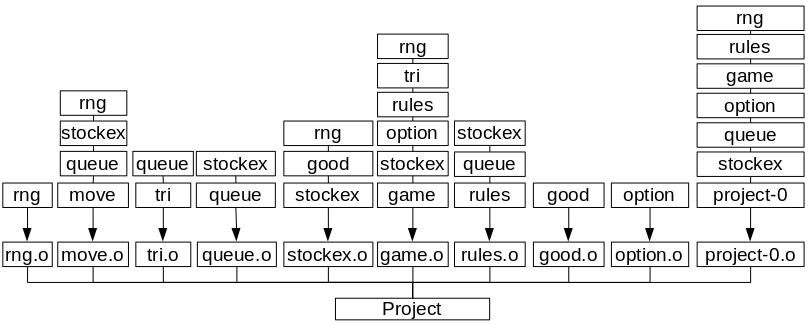
\includegraphics[scale=0.5]{Makefile.png}}
  \caption[le titre]{Makefile et D\'ependance}
\end{center}
\end{figure}
\subsection{Cr\'eation des structures et variables globales}

\subsubsection{Les constantes}

\begin{itemize}

\item Le prmier type de constantes mis en place sont les constntes qui vont \^etre utilis\'ees au cours du jeu, comme par exemple les differentes ressources,
qui sont d\'efinient dans le fichier \textbf{good.h}, ou bien comme les differentes places d'\'echanges, d\'efinient dans \textbf{stockex.h}.
\item Les autres constantes d\'efinient sont les constantes relatives aux r\`egles et limites du jeu, comme le nombre maximal de tours, de joueurs, ou bien de ressources. 
Ces constantes pourront \^etre entr\'ees comme argument lors de l'appelle de l'executable, et ainsi les parties seront personnalisable. 

\end{itemize} 

\subsubsection{Les structures}

\begin{itemize}

\item\textbf{Wallet}

La structure "Wallet" est la structure qui correspond au portefeille d'un joueur.
Elle est compos\'ee d'un tableau d'entiers, qui correspondent aux quantit\'es de chaque ressources que le joueur poss\`ede.

\begin{lstlisting}
// A wallet containing different amounts of goods
struct wallet 
{
  unsigned int data[MAX_GOOD];
};
\end{lstlisting}

\item\textbf{Stockex}

La structure "Stockex" est la structure qui correspond \`a une place d'\'echange.
Elle est compos\'e d'une chaine de caract\`ere, qui donne le nom de la place d'\'echange, d'un entier indiquant le nombre de transactions r\'ealisable dans cette place d'\'echange,
et enfin un tableau de transactions.

\begin{lstlisting}
// The type representing stock exchanges
struct stockex
{
  char name[MAX_STR];
  int nb_transac;
  struct transac transacs[MAX_TRANSAC];
};
\end{lstlisting}

\item\textbf{Transac}

La structure "Transac" est la structure qui correspond \`a une transaction.
Elle est compos\'e de deux portefeilles, qui corresepondent respectivement aux ressources venduent par la place d'\'echange, et \`a celle achet\'ees par cette m\^eme place d\'echange.

\begin{lstlisting}
// The type representing transactions
struct transac
{
  //The goods sold by the stockex
  struct wallet good_out;
  //The goods bought by the stockex
  struct wallet good_in;
};
\end{lstlisting}

\item\textbf{Queue}

La structure "Queue" est la structure qui correspond \`a la file de joueur
Elle est compos\'e d'une liste de pointeurs vers des joueurs, ainsi que le nomre de joueurs pr\'esent dans la file. 

\begin{lstlisting}
// This type represent a queue
struct queue
{
  struct teddy* list[MAX_PLYR]; 
  int nbr_of_teddies;
};
\end{lstlisting}

\item\textbf{Teddy}

La structure "Teddy" est la structure qui correspond \`a un joueur.
Elle est compos\'e d'un portefeuilles, d'un num\'ero d'identifiant, d'un temps de jeu, d'un nombre de ressource \'equivalent en "Honey", 
un nombre de places d'\'echanges visit\'ees, et une liste avec ces places d'\'echanges.

\begin{lstlisting}

// This type represent a teddy
struct teddy
{
  struct wallet wallet;
  int id;
  int time;
  int equiv_Honey;
  int nb__stockex_visited;
  struct sotckex visited__stockex[MAX_STOCKEX];
};
\end{lstlisting}

\end{itemize}

\subsection{Impl\'ementation d'une file de priorité}
Apr\'es la cr\'eation des structures et des variable globale, il faut mettre en place la file de priorit\'e, dans les fichiers \textbf{queue.[ch]}. Les teddies in\'eragissent avec les places d'\'echange en suivant un ordre de priorit\'e. La r\`egle dit qur le teddy prioritaire est celui avec le temps de jeu le plus faible. 
Donc la structure correspondant \`a un teddy comprend un portefeuille, un num\'ero d'identification, et un temps de jeu. 
La solution choisit pour mod\'eliser la file est une liste de pointeur vers des teddies, ainsi qu'un entier indiquant le nombre de teddies dans la file. 
Les fonctions cod\'es permettent de cr\'eer une file, ou bien d'int\'eragir avec la file, en faisant entrer un teddy, ou en faisant sortir le teddy prioritaire, et ainsi pouvoir le faire jouer. 
C'est aussi dans ce fichier qu'est d\'efinie le nombre maximal de joueur.
Les premiers probl\'emes rencontr\'es \'etaient li\'es \`a l'initialisation des teddies. Finalement, le code initialise les teddies un par un, et cr\'ee un tableau de pointeur vers ces derniers.
Ensuite, l'autre probl\`eme concerne la file et le classement des teddies dedans.
La solution adopt\'e est de ne s\'electionner que le teddy prioritaire, et de ne pas appliquer de classement sur le reste de la file. Le d\'efaut de cette m\'ethode est que la recherche du teddy prioritaire doit se faire \`a chaque tour.  

\subsection{Mise en place de la boucle de jeu}

Apr\'es avoir mis en place les differentes structures et la file de priorité, la boucle de jeu peut \^etre r\'ealis\'ee.
Le principe est de faire tourner la partie durant un temps pr\'ed\'efinie, tout en assurant le respect des r\`egles.
Au lancement de l'executable, il est possible de choisir certaine conditions, comme le nombre de joueurs, ou bien le nombre de tours. 
Donc pendant un tour de la partie, la prmi\'ere \'etape est de selectionner le joueur prioritaire, c'est \`a dire le joueur avec le temps de jeu le plus
faible. 
Ensuite il faut le faire choisir une transaction parmis celles propos\'ees par la place d'\'echange (Au d\'ebut du projet, il n'y avait qu'une seule place
d'\'echange) de mani\`ere al\'eatoire, puis ensuite il va r\'ealiser cette transaction un nombre de fois al\'eatoire que permet son portefeuille.
Une fonction qui permet d'avoir un nombre al\'eatoire entre des borns est alors implant\'ee. 
une fois la transaction r\'ealis\'ee, le joueur est sortie de la file, et replac\'e \`a la fin. Ce joueur ne joueura pas au tour suivant. 
\`A chaque tour, les joueurs doivent respecter r\`egles, sinon ils seront exclus.
Apr\'es le derniers tour du jeu, les r\'esultats des joueurs restant sont r\'ecup\'er\'es, les joueurs sont class\'es, et le classement est affich\'e. 


\subsection{Affichage des r\'esultats}

Une fois la partie termin\'ee, c'est à dire une fois que chaque teddy à un temps de jeu \'egal au temps de jeu maximal d\'efini en d\'ebut de partie; il faut afficher les r\'esultats.
Ainsi, la fonction 
\textit{display_results} 
se charge d'afficher le classement.
Pour chaque teddy restant, elle calcule l'\'equivalent-Honey de son 
\textbf{wallet},
puis elle effectue un tri 
\textbf{tri par insertion} 
sur la file de priorité compos\'ee des teddies.
Nous avons d\'ecid\'e de choisir ce tri car, m\^eme s'il est d'une complexit\'e asymptotique quadratique, il est en moyenne beaucoup plus rapide que le quicksort ou que tri fusion pour des jeux de données de petites tailles.
Or, notre projet s'effectue dans un contexte de 20 teddy maximum. \\
C'est donc pour cette raison que le tri que nous avons choisi d'impl\'ementer est le tri par insertion.

\section{R\'esultats}

\subsection{Base version} 

\subsubsection{Impl\'ementation des fichiers}

\begin{itemize}

\item\textbf{good.[ch] :} Les premiers fichiers mis en place sont les fichers good.[ch].
Les fichiers good vont d\'efinir les differentes ressources que peut acheter ou vendre un teddy, mais aussi la structure du portefeuille, le "wallet". 
A\' chaque ressource est associée une valeur.
C'est dans ce fichier qu'est d\'efinie la valeur maximale de ressources differentes.
Aucun probl\`eme n'a \'et\'e rencontr\'e pour coder good.[ch], mais il se peut que plus tard dans le projet il y ai des conflits, \`a cause de certaine modification de type. 

\item\textbf{stockex.[ch] :}  Les fichiers suivant ont \'et\'e les fichiers stockex.[ch], qui impl\'emente la notion de place d'\'echange, appell\'e ici les "stockex".
Une place d'\'echange va \^etre carat\'eris\'ee par une structure, contenant un nom,un nombre de transaction, et les transactions. 
Chaque transaction est d\'efinie par une portefeuille entrant, et un protefeuille sortant, aussi mod\'elis\'ee par une structure.
C'est dans ce fichier qu'est d\'efinie la valeur maximale de transactions differentes par place d'\'echange.
Lors de la mise en place des places d'\'echanges, les probl\`emes rencontr\'es sont principalement due \'a l'écriture des pointeurs, mais ils ont vite \'et\'e surmont\'es.
Pour le moment, une seule place d'\'echange est utilis\'ee, elle est d\'efinie dans le fichier stockex.h, d'apr\'es l'exemple de l'\'ennonc\'e mais il serait pertinent de coder une fonction qui permet de g\'en\'erer un stockex, avec des caract\'eristiques al\'eatoire.

\end{itemize}

\subsection{Achievement 1}

\section{Conclusion}

\end{document}